\chapter{General Introduction}
Particle Physics or sometimes called High Energy Physics, is the field of physics that pursues the ultimate structure of matter. This is possible in two ways, one is to look for elementary particles, the ultimate constituents of matter at their smallest scale. The other is to clarify what interactions are acting among the
\emph{(forces)} to construct matter.



\section{Large Hadron Collider (LHC)}

Hadron colliders are devices made to explore the world of particle physics, they work as theories testers and also as a discovery machines, an example of these hadron colliders is the Large Hadron Collider in CERN.

Inside the Large hadron Collider, $10^{11}$ protons are being accelerated to a high kinetic energy and then collided up 40 million times per second to provide 14 \si{TeV} proton-proton collision. The LHC also collides with heavy ions. Two general purpose detectors, ATLAS (A Toroidal LHC ApparatuS) and CMS (Compact Muon Solenoid) have been built for probing proton-proton and ion-ion collisions. \citep{Aad:2012tfa}.

The main mission of the LHC is to investigate the properties of the Higgs boson. The importance of the Higgs boson from investigating the validity of the standard model suggests that the masses of the elementary particles are generated through the Higgs mechanism. In July 2012, the ATLAS and CMS experiments at CERN's Large Hadron Collider announced that they have had each observed new particle in the mass region around 126 GeV. This particle is consistent with the Higgs boson predicted by the Standard Model.  
 
Most of the interesting physics at LHC involves investigating the results of these interactions (collisions). It has been observed that as a result of these collisions, stable partons are formed, partons consists of quarks and qluons. From experimental point of view, these collisions lead to the production of these partons along side the production of another particles like the $Higgs$ boson. However, new particles are not detected. Instead, the first parton (quark or gluon) that is being produced will produce more partons which  will also produce more partons and eventually leading to a spray of partons. This is called \textit{the parton shower}.      

The study of quarks and gluons in LHC is challenging because of the production of a single quark or a gluon will actually appear in the detectors as many particles collimated in the same general direction, all arriving at once. The detection of a collimated flow of particles of this nature is called a \textbf{jet} \citep{Ellis:2007ib}.   



\section{Quarks and Gluons}
In our current view, all matter is made of three kind of elementary particles, \emph{leptons}, \emph{quarks} and \emph{mediators}.

%Quarks and leptons are the building blocks which build up matter.
There are six "flavours" of quarks, these are up, down charm strange, top and bottom.
Quarks can successfully account for all known mesons and baryon which are known as hadrons,
%which are particles with spin $\frac{1}{2}$. Mesons consist of quark and anti quark for example the positive pion $\pi^+$ which consists of up and anti down quarks. Baryons consist of three quarks or three anti quarks for example the proton which consists of two up quarks and one down quark.
%
%
Quarks carry colour charge: red, green or blue, the colour name here is an analogy  that is famously used among physicists to describe a three kind of generating force. They are called by their number or any other index. We can also we think of it as a three primary additive colours. 

  
%Since all hadrons are colour charge neutral or colourless particles they have white charge. 
%
%Unlike other elementary particles quarks carry fractional charge and possess new quantum numbers.
%The table \ref{table1.1} summarizes some properties of quarks. Each quark flavour is associated with its own quantum number\footnote{These are the set of numbers that describes a conserved quantities in the dynamic of a quantum system, for example the set of numerical solutions of Schrödinger equation of the Hydrogen atom.}(the capital letters), those quantum numbers describes the decay of the particles, those first were meant to explain the fact that some particles decay slower than other particles, for example the first mentioned below the "Strangeness", it has been noticed that the higher the mass the lower the strangeness,  these numbers are conserved in strong and electromagnetic interactions but not in weak interaction, 
%These are: 
%\begin{itemize}
%\item[•]Strangeness: $S=-1$ for s-quark.
%
%\item[•]Charm: $C=+1$ for c-quark.
%
%\item[•]Beauty: $\tilde{B}=-1$ for b-quark. 
%
%\item[•] t - quark has life time too short to form hadrons. 
%\item[•]up and down quarks have nameless flavour quantum numbers.
%\end{itemize} \citep{particle}
%%\Jnote{What exactly is conserved here? Are these six values or just one?} 
%
%\begin{table}
%\begin{center} 
% \begin{tabular}{|c|c|c|c|} \hline 
%  Name (Flavour) & Symbol & Electric charge(in units of e) & Mass  \\ \hline 
%  $\text{Up}$ & $\text{u}$ &$ +\frac{2}{3}$ & $1.7-3.1 \frac{Mev}{c^2}$\\\hline
%  $\text{Down}$&$\text{d}$&$-\frac{1}{3}$& $4.1-5.7\frac{Mev}{c^2}$\\\hline
%  $\text{charm}$&$\text{c}$&$+\frac{2}{3}$&$1.18-1.34\frac{Gev}{c^2}$\\\hline
%  $\text{strange}$&$\text{s}$&$-\frac{1}{3}$&$80-130\frac{Mev}{c^2}$\\\hline
%  $\text{top}$&$\text{t}$&$+\frac{2}{3}$&$172.3-173.5\frac{Gev}{c^2}$\\\hline
%  $\text{bottom}$&$\text{b}$&$-\frac{1}{3}$&$4.13-4.37\frac{Gev}{c^2}$\\\hline
% \end{tabular}
%\caption{properties of Quarks}
%\label{table1.1}
%\end{center}
%\end{table}
%
%%\Jnote{Maybe extend the table to explain other properties of quarks?}
%
%\Jnote{Citations: If section(s) are based on a textbook, cite it in
%  the beginning, saying something like ``the following
%  presentation is based on \textbackslash cite\{...\}''}

%\section{Strong Force}
The other partons (glouns)  mediate the interaction between quarks. 
There are eight gluons, which come from the gauge group $SU(3)$ and has eight generators.

Gluon is a massless spin $1$ particle, carrying charge called colour charges as well as the quarks, because gluons can interact among themselves.
%Normally the range of the force can be calculated by a simple argument of the uncertainty\footnote{$\Delta E \Delta t \approx m c^2 \Delta t > \frac{\hbar}{2} \Longrightarrow range = c \Delta t > \frac{\hbar}{2 m c}$}, but this not the case for the strong force, the strong force is more complicated
%and involves a concept known as confinement.

The colour charge has strange property that it exerts a constant force that binds colour carrying particles together, this can be visualized using the analogy of a rubber band, the stronger you pull on the rubber band the tighter it feels.
If we do not pull on it at all, it hangs loose. The same thing happens for the particles,  that means at a very short distance, the force is relaxed and the particles behave as free particles. As the distance between them increases, the force acts like a rubber band and pulls them back stronger. When the rubber band is stretched beyond its limits, it cuts into many pieces producing more particles. This phenomenon is known as the colour confinement. In other words, these particles tend not to be separated by a macroscopic distance.
This limits the range of strong force, which is believed to be of order $10^{-15}\si{m}$ -
the dimension of a nuclear particle.

The theory which describes this force is called $Quantum$ $Chromodynamics$ \citep{particle}.

\section{Monte Carlo Simulation}

Due to the complex nature of the event\footnote{Event in this context refers to the result of the particle interaction (collision).} at the Large Hadrons Collider , the description of the final state involves a multi-particle calculations. The accurate prediction of the final state in hadron colliders is still one of the hardest problems. This problem roots to the non-abelian nature of QCD, which leads to a colour confinement at a long distance. The two main problems are the description of the hadron formation and the evolution of QCD final states from short to long distances. Those problems can be tackled to a good approximation by Monte-Carlo event generators.
The figure \ref{fig:parton} illustrates the collision of two protons and the splitting of the particles (parton shower) after the collisions.   

\begin{figure}[hbtp]
\centering
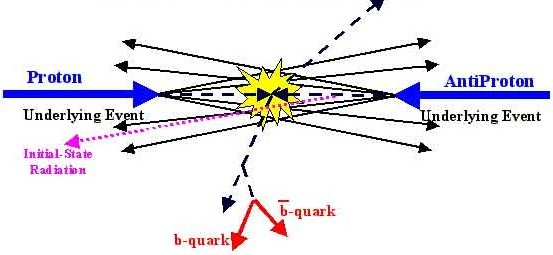
\includegraphics[scale=.7]{images/prd2_fragmentation.jpg}
\caption{Illustration of the parton shower}\label{fig:parton}
\end{figure}
